% $Header$
% MBDyn (C) is a multibody analysis code.
% http://www.mbdyn.org
%
% Copyright (C) 1996-2017
%
% Pierangelo Masarati  <masarati@aero.polimi.it>
%
% Dipartimento di Ingegneria Aerospaziale - Politecnico di Milano
% via La Masa, 34 - 20156 Milano, Italy
% http://www.aero.polimi.it
%
% Changing this copyright notice is forbidden.
%
% This program is free software; you can redistribute it and/or modify
% it under the terms of the GNU General Public License as published by
% the Free Software Foundation (version 2 of the License).
% 
%
% This program is distributed in the hope that it will be useful,
% but WITHOUT ANY WARRANTY; without even the implied warranty of
% MERCHANTABILITY or FITNESS FOR A PARTICULAR PURPOSE.  See the
% GNU General Public License for more details.
%
% You should have received a copy of the GNU General Public License
% along with this program; if not, write to the Free Software
% Foundation, Inc., 59 Temple Place, Suite 330, Boston, MA  02111-1307  USA

\section{Plate Elements}
\label{sec:EL:PLATE}


\subsection{Shell4}
\label{sec:EL:PLATE:SHELL4}

\emph{Authors: Marco Morandini and Riccardo Vescovini}

The shell4 elements model a four-node shell.
The syntax is
%\begin{verbatim}
\begin{Verbatim}[commandchars=\\\{\}]
    \bnt{elem_type} ::= \{ \kw{shell4eas} | \kw{shell4easans} \}

    \bnt{normal_arglist} ::=
        \bnt{node_1_label} , \bnt{node_2_label} , \bnt{node_3_label} , \bnt{node_4_label} ,
        \bnt{shell_constitutive_law_data}

    \bnt{shell_constitutive_law_data} ::=
        \{ [ \kw{matr} , ] \bnt{12x12_matrix}
            | \kw{sym} , \bnt{upper_triangular_12x12_matrix}
            | \kw{diag} , \bnt{diagonal_12x12_matrix}
            | \kw{isotropic} , \bnt{isotropic_data} \}
        [ , \kw{prestress} , (\ty{Vec12}) \bnt{prestress} ]

    \bnt{isotropic_data} ::=
        \{ \{ \kw{E} | \kw{Young modulus} \} , \bnt{E}
            | \{ \kw{nu} | \kw{Poisson modulus} \} , \bnt{nu}
            | \{ \kw{G} | \kw{shear modulus} \} , \bnt{G}
            | \kw{as} , \bnt{as}    # TODO: clarify
            | \kw{at} , \bnt{at}    # TODO: clarify
            | \kw{thickness} , \bnt{thickness} \}
        [ , ... ]
\end{Verbatim}
%\end{verbatim}
The names \kw{shell4eas} and \kw{shell4easans} respectively stand for
``Enhanced Assumed Strain'' (EAS)
and ``Enhanced Assumed Strain-Assumed Natural Strain'' (EAS-ANS).

Nodes are numbered according to Figure~\ref{fig:EL:PLATE:SHELL4:sketch}.
\begin{figure}
\centering
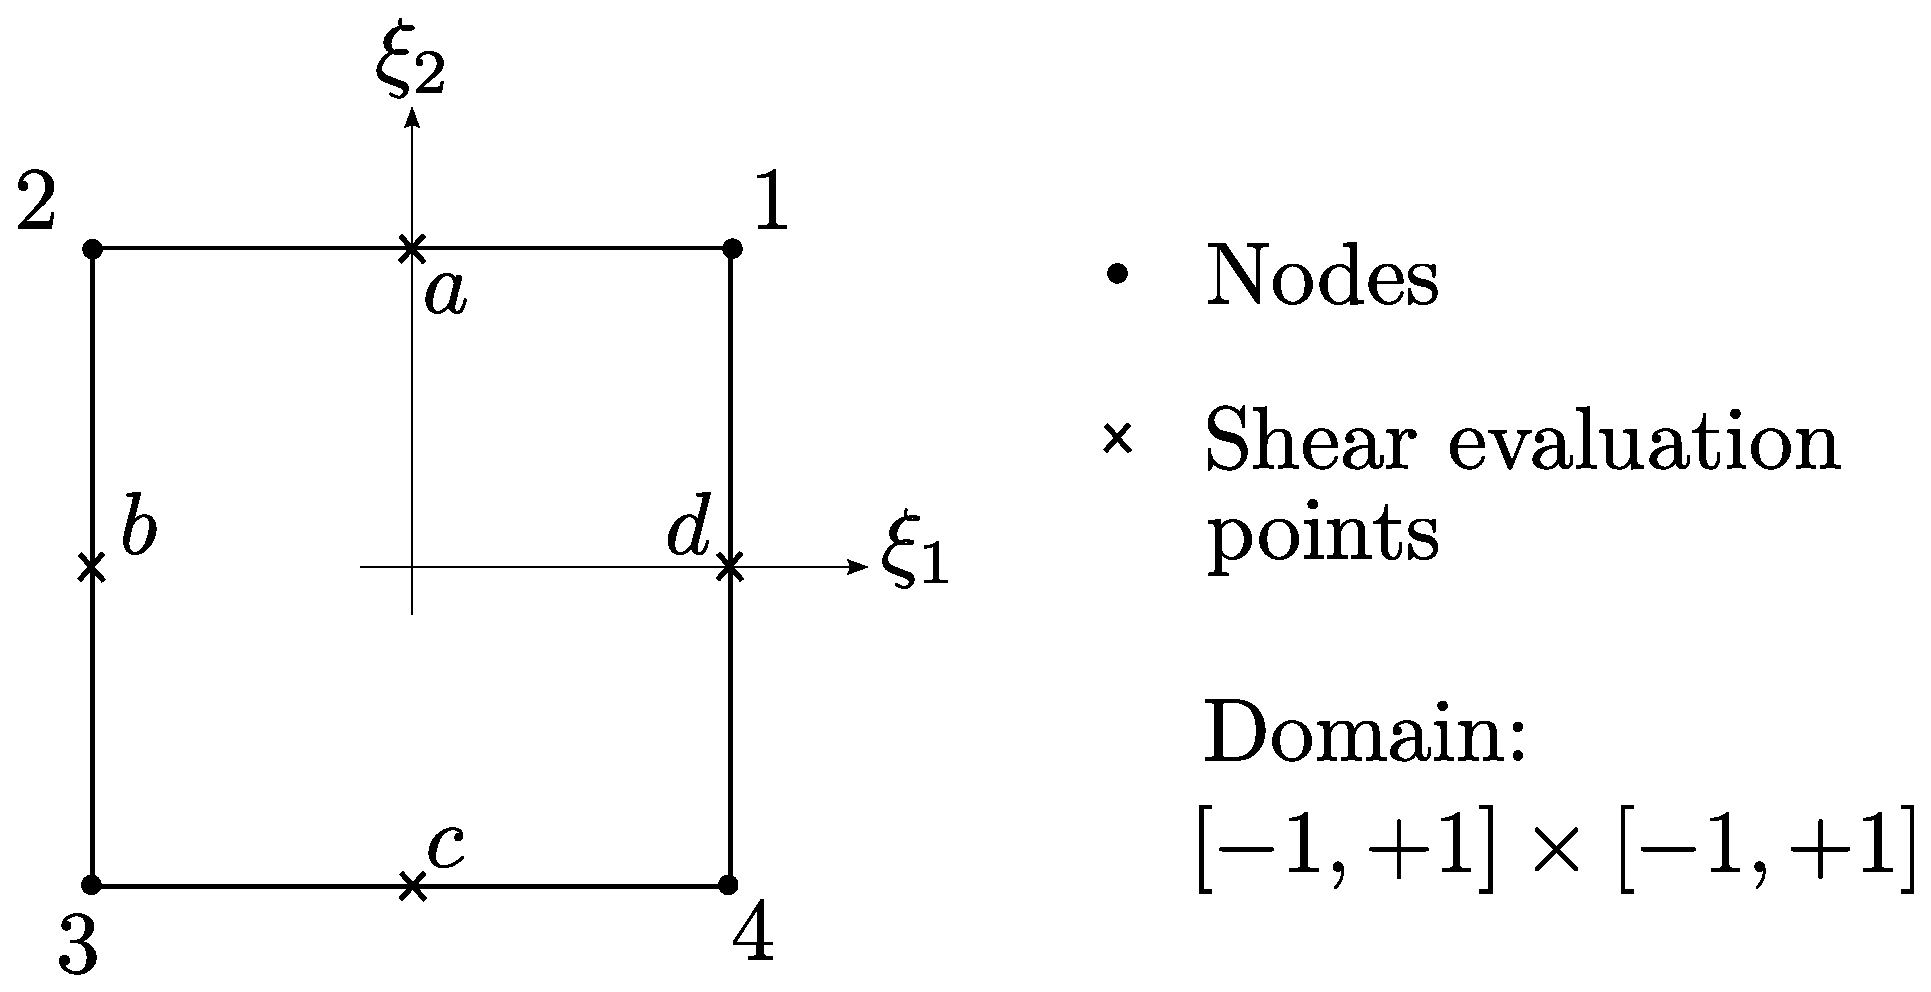
\includegraphics[width=.6\textwidth]{shellPic}
\caption{Shell: definitions}
\label{fig:EL:PLATE:SHELL4:sketch}
\end{figure}

Only linear elastic constitutive properties can be currently modeled.
They consist in a $12 \times 12$ matrix that expresses the force and moment
fluxes as functions of linear and angular strains according to
\begin{align}
	\cubr{\cvvect{
		n_{11} \\
		n_{12} \\
		n_{13} \\
		n_{21} \\
		n_{22} \\
		n_{23} \\
		m_{11} \\
		m_{12} \\
		m_{13} \\
		m_{21} \\
		m_{22} \\
		m_{23}
	}}
	&=
	\sqbr{D}
	\cubr{\cvvect{
		\varepsilon_{11} \\
		\varepsilon_{12} \\
		\varepsilon_{13} \\
		\varepsilon_{21} \\
		\varepsilon_{22} \\
		\varepsilon_{23} \\
		\kappa_{11} \\
		\kappa_{12} \\
		\kappa_{13} \\
		\kappa_{21} \\
		\kappa_{22} \\
		\kappa_{23}
	}}
	+
	\nt{prestress}
\end{align}
The \nt{prestress} is a force and moment per unit span contribution
to the force and moment fluxes.
Typically, only a membrane prestress makes sense, namely
\begin{Verbatim}[commandchars=\\\{\}]
    \bnt{prestress} ::= \bnt{T11} , \bnt{T12} , 0. , # force/span on face with normal 1
                    \bnt{T21} , \bnt{T22} , 0. , # force/span on face with normal 2
                    0.    , 0.    , 0. , # moment/span on face with normal 1
                    0.    , 0.    , 0.   # moment/span on face with normal 2
\end{Verbatim}
with $\nt{T21} \equiv \nt{T12}$.


When the \kw{isotropic} keyword is used, only two of the optional
sub-keywords \kw{E}, \kw{nu} and \kw{G} are required, as the remaining
parameter can be computed from the other two according to the relationship
\begin{align}
	\nt{G}
	&=
	\frac{\nt{E}}{2\plbr{1 + \nt{nu}}}
	.
\end{align}
If all are provided, they must be consistent.
The optional parameters \kw{as} and \kw{at} are not documented yet;
the default should be used.

When the (optional) \kw{matr} (or \kw{sym}) form is used,
the required data for an orthotropic plate, from Classical Laminate Theory (CLT),
with the principal axes of orthotropy parallel to the edges of the structure and laminate,
and with a symmetrical arrangement of the layers, are
\begin{align}
        \cubr{\cvvect{
                N_{x}
                \\
                N_{y}
                \\
                N_{xy}
                \\
                M_{x}
                \\
                M_{y}
                \\
                M_{xy}
        }}
        &=
        \sqbr{\matr{cccccc}{
	 CE_{x} & C\nu_{xy}E_y & 0 & 0 & 0 & 0 
	 \\
	 C\nu_{xy}E_y & CE_{y} & 0 & 0 & 0 & 0 
	 \\
	 0 & 0 & 2G_{xy}h & 0 & 0 & 0 
	 \\
	 0 & 0 & 0 & DE_{x} & D\nu_{xy}E_y & 0
	 \\
	 0 & 0 & 0 & D\nu_{xy}E_y & DE_{y} & 0 
	 \\
	 0 & 0 & 0 & 0 & 0 & 2F 
	        }}
        \cubr{\cvvect{
                \varepsilon_{x}
                \\
                \varepsilon_{y}
                \\
                \varepsilon_{xy}
                \\
                \kappa_{x}
		\\
                \kappa_{y}
		\\
                \kappa_{xy}
        }}
\end{align}
with
\begin{subequations}
\begin{align}
	C &= \frac{h}{1-\nu_{xy}\nu_{yx}}
	\\
	D &= \frac{h^3}{12(1-\nu_{xy}\nu_{yx})}
	\\
	F &= \frac{G_{xy}h^3}{12} 
\end{align}
\end{subequations}
The data actually required by MBDyn are
{\tiny
\begin{align}
        \cubr{\cvvect{
                N_{11}
                \\
                N_{12}
                \\
                N_{13}
                \\
                N_{21}
                \\
                N_{22}
                \\
                N_{23}
                \\
                M_{11}
                \\
                M_{12}
                \\
                M_{13}
		\\
                M_{21}
                \\
                M_{22}
                \\
                M_{23}
        }}
        &=
        \sqbr{\matr{cccccccccccc}{
  CE_{x} & 0      & 0      & 0 & C\nu_{xy}E_y & 0     & 0 & 0 & 0 & 0 & 0 & 0
  \\                                                                                
  0      & 2G_{xy}h  & 0   & 0 & 0  & 0               & 0 & 0 & 0 & 0 & 0 & 0
  \\                                                                             
  0      & 0      & \alpha_sG_{xy}h      & 0      & 0      & 0      & 0 & 0 & 0 & 0 & 0 & 0
  \\                                                                             
  0      & 0 & 0      & 2G_{xy}h & 0 & 0      & 0 & 0 & 0 & 0 & 0 & 0
  \\                                                                             
  C\nu_{xy}E_y & 0 & 0      & 0 & CE_{y} & 0      & 0 & 0 & 0 & 0 & 0 & 0
  \\                                                                             
  0      & 0      & 0      & 0      & 0      & \alpha_sG_{xy}h      & 0 & 0 & 0 & 0 & 0 & 0
  \\                                                                                                      
  0 & 0 & 0 & 0 & 0 & 0      & 2F & 0 & 0    & 0 & 0 & 0
  \\                                                                                                 
  0 & 0 & 0 & 0 & 0 & 0      & 0 & DE_x & 0    & -D\nu_{xy}E_y & 0 & 0
  \\                                                                                                 
  0 & 0 & 0 & 0 & 0 & 0      & 0      & 0        & 2F\alpha_t    & 0        & 0      & 0
  \\                                                                                                 
  0 & 0 & 0 & 0 & 0 & 0      & -D\nu_{xy}E_y & 0 & 0    & DE_y & 0 & 0
  \\                                                                                                 
  0 & 0 & 0 & 0 & 0 & 0      & 0 & 0 & 0    & 0 & 2F & 0
  \\                                                                                                 
  0 & 0 & 0 & 0 & 0 & 0      & 0      & 0        & 0    & 0        & 0      & 2F\alpha_t
        }}
        \cubr{\cvvect{
                \varepsilon_{11}
                \\
                \varepsilon_{12}
                \\
                \varepsilon_{13}
                \\
                \varepsilon_{21}
                \\
                \varepsilon_{22}
                \\
                \varepsilon_{23}
                \\
                \kappa_{11}
		\\
                \kappa_{12}
		\\
                \kappa_{13}
                \\
                \kappa_{21}
		\\
                \kappa_{22}
		\\
                \kappa_{23}
        }}
\end{align}
}

\noindent
where $\alpha_s$ is the shear factor, and the torsional factor $\alpha_t$ 
is the material coefficient typical for a 6-field shell theory, which does not appear in conventional shell theories.
It should be viewed as an analogue of the shear factor. 
Values of $\alpha_t$  from 0 to 1 have negligible influence on displacements and on the internal energy of the system.
See \cite{WITKOWSKI-2009-EAS-ANS} for details.

% \textbf{TODO: improve}



\subsection{Membrane4}
\label{sec:EL:PLATE:MEMBRANE4}

\emph{Authors: Marco Morandini and Tommaso Solcia}

The membrane4 element models a four-node membrane.
The syntax is
%\begin{verbatim}
\begin{Verbatim}[commandchars=\\\{\}]
    \bnt{elem_type} ::= \kw{membrane4eas} 

    \bnt{normal_arglist} ::=
        \bnt{node_1_label} , \bnt{node_2_label} , \bnt{node_3_label} , \bnt{node_4_label} ,
        \bnt{membrane_constitutive_law_data}

    \bnt{membrane_constitutive_law_data} ::=
        \{ [ \kw{matr} , ] \bnt{3x3_matrix}
            | \kw{sym} , \bnt{upper_triangular_3x3_matrix}
            | \kw{diag} , \bnt{diagonal_3x3_matrix}
            | \kw{isotropic} , \bnt{isotropic_data} \}
        [ , \kw{prestress} , (\hty{Vec3}) \bnt{prestress} ]

    \bnt{isotropic_data} ::=
        \{ \{ \kw{E} | \kw{Young modulus} \} , \bnt{E}
            | \{ \kw{nu} | \kw{Poisson modulus} \} , \bnt{nu}
            | \{ \kw{G} | \kw{shear modulus} \} , \bnt{G}
            | \kw{thickness} , \bnt{thickness} \}
        [ , ... ]
\end{Verbatim}
%\end{verbatim}
The name \kw{membrane4eas} stands for ``Enhanced Assumed Strain'' (EAS).
Nodes are numbered according to Figure~\ref{fig:EL:PLATE:SHELL4:sketch}.
Only linear elastic constitutive properties can be currently modeled.
They consist in a $3 \times 3$ matrix that expresses the force
fluxes as functions of linear strains according to
\begin{align}
	\cubr{\cvvect{
		n_{11} \\
		n_{22} \\
		n_{12}
	}}
	&=
	\sqbr{D}
	\cubr{\cvvect{
		\varepsilon_{11} \\
		\varepsilon_{22} \\
		\varepsilon_{12}
	}}
	+
	\nt{prestress}
\end{align}
The \nt{prestress} is a force per unit span contribution
to the force fluxes,
\begin{Verbatim}[commandchars=\\\{\}]
    \bnt{prestress} ::= \bnt{T11} , \bnt{T22} , \bnt{T12}
\end{Verbatim}

When the \kw{isotropic} keyword is used, only two of the optional
sub-keywords \kw{E}, \kw{nu} and \kw{G} are required, as the remaining
parameter can be computed from the other two according to the relationship
\begin{align}
	\nt{G}
	&=
	\frac{\nt{E}}{2\plbr{1 + \nt{nu}}}
	.
\end{align}
If all are provided, they must be consistent.


When the (optional) \kw{matr} (or \kw{sym}) form is used,
the required data for an orthotropic membrane are

\begin{align}
        \cubr{\cvvect{
                N_{11}
                \\
                N_{22}
                \\
                N_{12}
        }}
        &=
        \sqbr{\matr{cccccc}{
	 CE_{1} & C\nu_{21}E_1 & 0  
	 \\
	 C\nu_{12}E_2 & CE_{2} & 0  
	 \\
	 0 & 0 & 2G_{12}h  
       }}
        \cubr{\cvvect{
                \varepsilon_{11}
                \\
                \varepsilon_{22}
                \\
                \varepsilon_{12}
        }}
\end{align}
with
\begin{subequations}
\begin{align}
	C &= \frac{h}{1-\nu_{12}\nu_{21}}
	\\
	\nu_{12}E_2 &= \nu_{21}E_1 
\end{align}
\end{subequations}

\paragraph{Example:}
\begin{verbatim}
    membrane4eas: 100, 1, 2, 3, 4,
        matr, E1*H/(1-NU12*NU21),      E1*H*NU21/(1-NU12*NU21), 0,
              E2*NU12*H/(1-NU12*NU21), E2*H/(1-NU12*NU21),      0,
              0,                       0,                       2*G12*H,
        prestress, PS, PS, 0.;
\end{verbatim}


